\chapter{Derivadas}


\section{La Regla de L'Hôpital}

Una de las situaciones más frecuentes al calcular límites es la aparición de \emph{formas indeterminadas}: expresiones del tipo $\frac{0}{0}$ o $\frac{\infty}{\infty}$ que por sí solas no determinan el valor del límite. Para resolverlas, existe una herramienta poderosa debida a Guillaume de l'Hôpital ---aunque frecuentemente atribuida a Johann Bernoulli, quien la descubrió y la comunicó a l'Hôpital---: el criterio que lleva su nombre.

\begin{theorem}[Regla de L'Hôpital]
Sea $\lim_{x \to c} f(x) = 0$ y $\lim_{x \to c} g(x) = 0$ (o ambos infinitos). Si $f$ y $g$ son diferenciables en un entorno de $c$ (salvo posiblemente en $c$), $g'(x) \neq 0$ en ese entorno, y $\lim_{x \to c} \frac{f'(x)}{g'(x)}$ existe, entonces
\[
\lim_{x \to c} \frac{f(x)}{g(x)} = \lim_{x \to c} \frac{f'(x)}{g'(x)}.
\]
\end{theorem}

\begin{example}
Calcular $\lim_{x \to 0} \frac{x - \sin x}{x^3}$.
\end{example}

\begin{myproof}
La sustitución directa produce $\frac{0}{0}$, una forma indeterminada. Aplicamos la regla de L'Hôpital repetidamente:
\[
\lim_{x \to 0} \frac{x - \sin x}{x^3} = \lim_{x \to 0} \frac{1 - \cos x}{3x^2} = \lim_{x \to 0} \frac{\sin x}{6x} = \frac{1}{6} \lim_{x \to 0} \frac{\sin x}{x} = \frac{1}{6} \cdot 1 = \frac{1}{6}.
\]
\end{myproof}

\begin{rem}
La regla de L'Hôpital es aplicable también a formas indeterminadas del tipo $0 \cdot \infty$, $\infty - \infty$, $0^0$, $1^\infty$ e $\infty^0$, tras una reescritura algebraica adecuada que las reduzca a la forma $\frac{0}{0}$ o $\frac{\infty}{\infty}$.
\end{rem}

\section{Ejercicios}

\begin{prob}
Encuentre la ecuación de la recta perpendicular a la recta tangente en el punto $(1, 2)$ sobre la gráfica de $f(x) = -4x^2 + 6x$.
\end{prob}

\begin{prob}
Dado el polinomio cúbico $f(x) = x^3 - 3x^2 - 9x + 5$:
\begin{itemize}
    \item \textbf{Verifique} que los puntos $(-1, 10)$ y $(3, -22)$ pertenecen a la curva.
    \item \textbf{Demuestre} que la recta tangente a $f$ en cada uno de esos puntos es horizontal.
    \item \textbf{Grafique} el polinomio y las rectas tangentes horizontales en los puntos dados.
\end{itemize}
\end{prob}

\begin{prob}
Sea $y = \sqrt{x}$.
\begin{enumerate}[a)]
    \item Halle la pendiente de la recta tangente en $x = a$.
    \item Halle las ecuaciones de las rectas tangentes en los puntos $(1, 1)$ y $(4, 2)$.
\end{enumerate}
\end{prob}

\begin{prob}
Halle la ecuación de la recta tangente a $y = f(x)$ en $x = 5$, sabiendo que $f(5) = 3$ y $f'(5) = 4$.
\end{prob}

\begin{prob}
Dibuje la gráfica de una función $f$ para la cual $f(0) = 0$, $f'(0) = 3$, $f(1) = 0$ y $f(2) = 1$.
\end{prob}

\begin{prob}
Si se lanza una roca verticalmente hacia arriba en el planeta Marte con una velocidad inicial de $10~\text{m/s}$, su altura (en metros) después de $t$ segundos es $H(t) = 10t - 1.86t^2$.
\begin{enumerate}[a)]
    \item Halle la velocidad de la roca después de un segundo.
    \item Halle la velocidad de la roca cuando $t = a$.
    \item ¿Cuándo caerá la roca a la superficie?
    \item ¿Con qué velocidad chocará la roca contra la superficie?
\end{enumerate}
\end{prob}

\begin{prob}
Suponga que un círculo de radio $r$ y centro $(0, c)$ está inscrito en la parábola $y = x^2$ como lo muestra la siguiente figura. En el punto de tangencia, las pendientes de ambas curvas deben coincidir. Encuentre la pendiente de la circunferencia implícitamente y muestre que en el punto de tangencia $y = c - \dfrac{r^2}{2}$. Luego use las ecuaciones de la circunferencia y la parábola para mostrar que $c = r^2 + \dfrac{1}{4}$.

\begin{center}
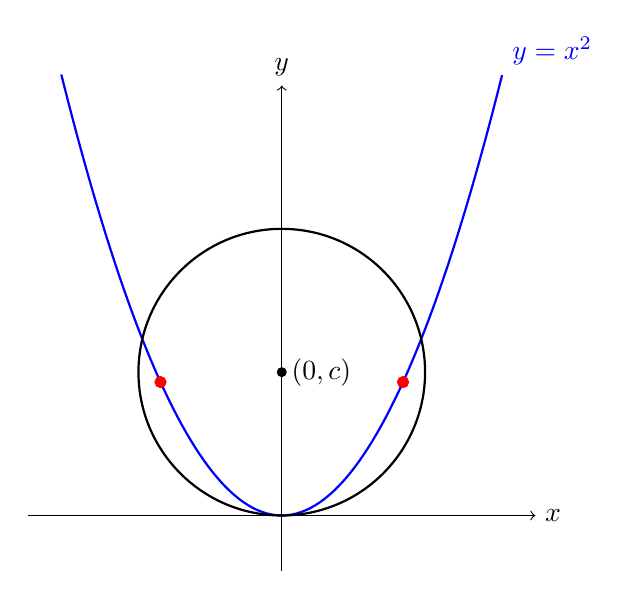
\begin{tikzpicture}[scale=1.4]
  \draw[->] (-2.3,0) -- (2.3,0) node[anchor=west] {$x$};
  \draw[->] (0,-0.5) -- (0,3.9) node[anchor=south] {$y$};
  \draw[blue,thick,domain=-2:2,samples=100] plot (\x,{\x*\x})
    node[above right] {$y = x^2$};
  \draw[thick] (0,1.3) circle [radius=1.3];
  \filldraw (0,1.3) circle (0.04) node[right] {$(0, c)$};
  \filldraw[red] (1.1,{1.1*1.1}) circle (0.05);
  \filldraw[red] (-1.1,{1.1*1.1}) circle (0.05);
\end{tikzpicture}

\textit{Figura: Un círculo de radio $r$ inscrito en la parábola $y = x^2$.}
\end{center}
\end{prob}